\documentclass{article}
\usepackage[final]{nips_2017}
\usepackage[utf8]{inputenc} % allow utf-8 input
\usepackage[T1]{fontenc}    % use 8-bit T1 fonts
\usepackage{hyperref}       % hyperlinks
\usepackage{url}            % simple URL typesetting
\usepackage{booktabs}       % professional-quality tables
\usepackage{amsfonts}       % blackboard math symbols
\usepackage{amsmath}
\usepackage{nicefrac}       % compact symbols for 1/2, etc.
\usepackage{microtype}      % microtypography
\usepackage{graphicx}
\usepackage{natbib}
\usepackage{listings}
\usepackage{xcolor}
\usepackage{pgfplots}
\usepackage{tikz}
\usepackage{subcaption}
\usepackage{multirow}
\usepackage{cellspace}

% bib keys (all present in sample.bib, all cited): shao2024deepseekmath, saab2025medgemma, hu2022lora,
%   chen2024huatuogpto1, zhang2025medrlvr, lin2025ehrmind, liu2021dream, ng1999shaping, andrychowicz2017her

\title{When Verifiable RL Helps Clinical Information Gathering:\\
Capability Gates, SFT Coverage, and Reward Geometry}

\author{
  Brendan P. Murphy \\
  \texttt{csbrendan@gmail.com} \\
}

\begin{document}
\maketitle

\begin{abstract}
We study \emph{when} reinforcement learning with verifiable rewards (RLVR)
improves adaptive clinical information-gathering --- asking the decision-relevant
questions before committing to an action --- and \emph{when} it instead degrades
safety. Across three stylized but structurally distinct medical tasks
(medication-refill triage, acute diagnostic work-up, and dosing titration), we
find that two cheap pre-RL \emph{gates} --- a demonstrability gate (does adaptive
gathering beat any fixed policy?) and a latent-support gate (can the model sample
the optimal behavior?) --- are \emph{necessary but not sufficient}. Even when both
gates pass, plain Group Relative Policy Optimization (GRPO) trained on the outcome
reward learns \emph{unsafe shortcut policies}: one-question collapse,
under-gathering, and defensive hedging that raise mean reward while
\emph{regressing} performance on the rare, safety-critical high-risk cases. An
information-gain credit-assignment reward --- dense credit for asks that reduce
uncertainty about the latent state, applied only in the RL rollout so the gates
stay pure --- recovers safer high-risk behavior and is \emph{thesis-positive} on
diagnostics, and a decoupled explore/exploit variant pushes high-risk
oracle-grade support to $1.00$ at a characterizable over-gathering cost. We show
the credit coefficient is itself a task-specific safety dial with a narrow
optimum: too small and the policy under-gathers, too large and it over-gathers.
SFT-initialized experiments show RL's benefit tracks the \emph{headroom} the
supervised model leaves: where a warmup already saturates the safety-critical
behavior, RL adds little, and --- testing the common case of an SFT trained on
incomplete data --- RL does \emph{not} reliably repair a high-risk coverage gap.
Re-measuring the latent-support gate on the biased SFT predicts repairability, but
satisfying it is necessary, not sufficient: from a strong biased initialization
both rewards re-shortcut (one under-gathering, one over-gathering) rather than
repair. Our contribution is a mechanism and a
practical recipe --- gate before training, then shape the reward to credit
gathering --- for predicting and controlling whether RL makes clinical decision
agents safer or merely game the verifier. The environments are stylized; the claim
is about RL learning dynamics under verifiable reward, not clinical deployment.
\end{abstract}


\section{Introduction}
\label{sec:intro}

Much of clinical decision-making is an \emph{adaptive information-gathering}
process, not a one-shot classification. A clinician adjusting a chronic
medication, triaging a refill, or working up an acute presentation first elicits
the decision-relevant facts --- current symptoms, recent labs, adherence,
contraindications --- and commits only once enough is known. The skill that
matters is \emph{which} questions to ask for this patient, asked efficiently, and
\emph{when} enough has been gathered to act safely. This gather-then-commit
trade-off is precisely the kind of policy choice that supervised imitation
captures poorly and that reinforcement learning (RL) is designed to optimize,
which makes RLVR --- recently extended from math and code to medicine
\citep{chen2024huatuogpto1, zhang2025medrlvr, lin2025ehrmind} --- an attractive
post-training tool for clinical agents.

But ``RL can help'' is the wrong question, and a dangerous default in a safety
context. The right questions are \emph{when} RL helps and, more importantly,
\emph{how it can hurt}. Our central finding is that on clinical gathering tasks
the binding constraint is not model \emph{capability} but \emph{reward geometry}:
with the obvious outcome reward, RL does not learn careful gathering --- it learns
\emph{shortcuts} that maximize the verifier while abandoning the behavior the task
was built to elicit. Two shortcuts recur and both are clinically unsafe: the
policy collapses to asking a single question (or none) and guessing, or it
defensively hedges to a ``safe'' middle action that scores acceptably on average
while losing the ability to identify and correctly treat the rare emergency.
Mean reward goes \emph{up} while safety-critical performance goes \emph{down} ---
so mean reward is a misleading scoreboard, and a naive RL pipeline can ship a
\emph{less} safe policy than it started with.

We make three contributions. (1) We define two analytic, training-free
\emph{gates} that predict, before any policy-gradient compute is spent, whether RL
can help at all: a \emph{demonstrability} gate (does adaptive gathering strictly
beat the best fixed policy?) and a \emph{latent-support} gate (can the
initialization policy even sample the optimal behavior?). (2) Across three
structurally distinct medical tasks we show these gates are \emph{necessary but
not sufficient}: passing them does not earn an RL win, because plain GRPO finds
the unsafe shortcuts above. We show that an explicit \emph{information-gain
credit-assignment} reward is the missing ingredient that converts a gates-passing
task from exploited to safely adaptive, that a decoupled explore/exploit scheme
further improves the safety-critical subset, and that the credit coefficient is a
task-specific dial with a narrow safe optimum. (3) We add a small SFT-vs-RL bridge
showing RL's benefit tracks the headroom a supervised initialization leaves ---
giving a practical decision recipe for when to run RL, and how to shape its reward
so it improves rather than games clinical safety.

We deliberately study \emph{stylized, verifiable} environments. Each task is an
adaptive value-of-information (VOI) partially observed decision process whose
reward is an exact analytic verifier, so we can measure demonstrability, latent
support, and shortcut exploitation directly rather than inferring them from a
learned reward model. This trades clinical realism for clean isolation of the
mechanism --- reward shape vs.\ safe gathering --- and follows a long line of
controlled-environment RL studies; the contribution is the mechanism and the
recipe, not a deployment-validated policy.


\section{Background}
\label{sec:background}

\paragraph{Adaptive gathering as a verifiable POMDP.} We model each task as an
ask$\,\to\,$commit dialogue over a partially observed case. A hidden latent state
$\mu$ (true severity, or a joint clot/bleed risk) is fixed by binary findings the
model may query one at a time; each answered query reveals a finding at a small
per-ask cost, and the episode ends at a single committed action. The reward is
verifiable and analytic,
$R = U[\,\text{true state}\,][\,\text{action}\,] - c\cdot n_{\text{asks}}$,
with $U$ a hand-specified utility matrix and $c$ the per-ask cost. Because $U$ and
the finding priors are known in simulation, we compute the exact adaptive oracle,
the best fixed (no-gathering) policy, and the posterior over $\mu$ given any
revealed set --- the quantities the gates and the credit-assignment signal need.
The optimizer is GRPO \citep{shao2024deepseekmath}; the base model is the compact
clinical \texttt{medgemma-4b-it} \citep{saab2025medgemma} with LoRA adapters
\citep{hu2022lora}.

\paragraph{Two gates: predict where RL can help, before spending compute.} A
recurring failure of applied RLVR is spending compute where RL cannot beat
supervised learning. We screen every task with two cheap gates --- one analytic,
one inference-only --- before committing any policy-gradient compute.

\emph{Gate~1 --- demonstrability (behavioral-cloning gap).} We require the adaptive
oracle to strictly beat the best fixed-action policy:
$\text{BC-gap} = V_{\text{oracle}} - \max_a \mathbb{E}[U[\mu][a]] > 0$. If a single
fixed action is near-optimal, gathering is pointless and imitation already
suffices --- the regime where a prior multi-turn study found RL flat. A positive
BC-gap is necessary for adaptive gathering to have value.

\emph{Gate~2 --- latent support.} We require that the policy initializing RL can
\emph{realize} the oracle action under sampling --- measured as support@$k$, the
fraction of cases for which at least one of $k$ temperature rollouts gathers and
commits to an oracle-grade action. That initialization is the base model where it
is already strong enough (diagnostics and titration here train from base), or a
light SFT warmup where the base cannot sample the optimum (refill triage). If the
optimal behavior is never sampled even after warmup, RL has no positive signal to
reinforce --- the ``knowledge absent'' failure that motivates an SFT warmup before
RL \citep{lin2025ehrmind}.

Neither gate requires an RL-training run --- that is the point of gating
\emph{before} spending policy-gradient compute, not that the probed model is
untrained. Gate~1 needs no model at all (it is analytic, from $U$ and the priors);
Gate~2 is a single forward-pass support probe of the initialization policy (base
or SFT warmup). Both depend only on the \emph{environment} ($U$, priors) and the
fixed RL-initialization policy, never on any reward shaping we add for RL; we keep
all shaping out of $U$ and the gates so gate measurements remain a clean,
shaping-independent description of the task.

\paragraph{Training structured inference procedures.} Recent RL methods increasingly
train models not merely to produce a single correct reasoning trace, but to use
structured inference-time compute. SPIRAL \citep{hamid2026spiral} trains a language
model to coordinate sequential reasoning, parallel search traces, and aggregation,
optimizing the full search-and-aggregate pipeline against the final reward. This is
complementary to our setting: rather than training parallel trace aggregation, we
study a different structured inference primitive --- adaptive clinical information
gathering before commitment. In safety-critical clinical tasks the desired object is
not merely a correct final answer but a structured procedure: gather relevant facts,
compare alternatives, resolve uncertainty, and only then commit to an action. (We
cite SPIRAL as conceptual support for the broader move toward training structured
inference procedures; it is math/reasoning work, not medical, and not evidence for
clinical safety.)

\paragraph{Denser feedback than sparse outcome rewards.} Recent work has also
explored alternatives to sparse outcome-reward RLVR that preserve on-policy training
while providing denser feedback. \citet{zhao2026selfdistilledreasoner} introduce
On-Policy Self-Distillation (OPSD), where the same LLM plays both student and
teacher: the student generates an on-policy response from the problem alone, while
the teacher conditions on privileged reference solutions and provides token-level
distributional supervision along the student's rollout. OPSD is not conventional
RLVR, but it targets the same credit-assignment weakness of sequence-level rewards
that motivates our work: GRPO supplies a sparse final-answer signal, whereas OPSD
provides dense feedback even when the final answer is wrong. Our approach is
complementary --- rather than using privileged reference traces for token-level
self-distillation, we use an analytic verifier to assign dense information-gain
credit to clinically useful questions during RL.

\paragraph{Medical multi-turn agents and RL for clinical consultation.} Closest in
application are recent medical dialogue agents that use RL to train proactive
clinical questioning. \citet{feng2026doctoragentrl} introduce DoctorAgent-RL, a
multi-agent framework in which a doctor agent interacts with an LLM-based patient
agent and receives evaluator rewards for diagnostic accuracy, information
acquisition, and protocol compliance; their MTMedDialog dataset supports dynamic
patient simulation through hidden patient profiles, and their SFT+GRPO pipeline
trains a Qwen2.5-7B doctor agent to ask strategic questions before diagnosis. This
work strongly supports the premise that clinical consultation should be modeled as
an adaptive information-gathering process rather than a single-turn
answer-generation task. Our work is complementary: DoctorAgent-RL demonstrates an
applied end-to-end medical consultation system, whereas we isolate the RL learning
dynamics in controlled verifiable environments, asking when gates, SFT coverage, and
reward geometry make RL improve safe gathering versus exploit shortcuts such as
under-gathering, one-question collapse, or defensive hedging.


\section{Methods}
\label{sec:method}

\subsection{Plain GRPO and the unsafe-shortcut problem}
We train bounded, fully on-policy GRPO from the base model or a light SFT warmup,
on a disaggregated two-node stack (training node plus a separate vLLM rollout
server) with an \texttt{env\_mask} that excludes simulator tokens from the policy
gradient so only model-generated tokens are trained. The trajectory reward is the
verifiable $R$ above. Even on tasks that \emph{pass both gates}, plain GRPO
converges to reward-equivalent shortcuts rather than adaptive gathering. Two modes
recur, both unsafe: (i) \emph{one-ask collapse / under-gathering} --- the policy
asks one question (or none) and commits, trimming gathering toward a fixed
checklist; and (ii) \emph{defensive hedging} --- the policy commits a ``safe''
middle action that scores acceptably on average but abandons the ability to
identify and treat the high-stakes minority. Both raise mean reward while
destroying the safety-critical behavior, so we never judge by mean reward alone.
We evaluate with a \emph{guarded report} that audits per-subset behavior and emits
one of several verdicts --- \textsc{thesis-positive}, \textsc{exploit}
(ask-collapse or high-risk regression), or \textsc{termination-only} (reward rose
only by learning to commit, not by gathering better).

\subsection{Information-gain credit assignment}
The shortcut problem is one of credit assignment: the terminal reward does not
tell the policy \emph{which ask} produced a good commit, so the cheapest way to
raise reward is to stop asking. We address it directly with a dense
\emph{information-gain} reward --- an intrinsic reward for uncertainty reduction,
in the spirit of potential-based reward shaping \citep{ng1999shaping}: each new,
decision-relevant ask is rewarded in proportion to the entropy reduction of the
posterior over the latent state,
$\Phi = -\,\Delta H\big(p(\mu \mid \text{revealed})\big)$, summed over the asks and
added to the terminal reward with weight $\lambda$. Irrelevant or repeated asks
reduce no entropy and earn nothing, so the signal rewards \emph{useful} gathering
specifically. It is computed from the same analytic posterior the gates use, but
applied \emph{only} in the RL rollout reward --- never in $U$, in
\texttt{env.score}, or in the gates --- so baseline comparisons and gate
measurements stay pure. This is ordinary per-ask credit assignment within a single
policy and a single episode; it densifies the gathering signal but does
\emph{not} separate exploration from exploitation. The decoupled variant below
does.

\subsection{DREAM-style decoupled exploration and exploitation}
The information-gain reward shares one policy and one trajectory across asking and
committing, so the two still compete for the same gradient. The DREAM line of
meta-RL \citep{liu2021dream} decouples them; we adapt that idea with a
\emph{single network and adapter} (no learned decoder, no second policy) and a
mode token: an \emph{explore} phase that may only ask, rewarded by recoverability
of $\mu$ (the information-gain signal), and an \emph{exploit} phase that commits
over \emph{only} the explore-gathered findings, rewarded by the pure verifiable
$U$. Decoupling is realized by alternating which phase receives the gradient
update across steps, so the two rewards are advantage-normalized within their own
phase. At deployment the composed policy runs explore$\,\to\,$gather$\,\to\,$commit
as a single dialogue, evaluated \emph{only} in that composed form --- a hard guard
ensures the commit phase never sees the privileged latent, so reported numbers
reflect a deployable policy.

\subsection{SFT-then-RL: initialization and coverage}
\label{subsec:bridge}
The industrially standard pipeline is SFT \emph{then} RL, which raises the question
of when RL adds value \emph{over} a supervised initialization. Our three main tasks
isolate reward geometry by training RL from base (diagnostics, titration) or a
light warmup (refill triage). We add two SFT-initialized probes of how
initialization and \emph{data coverage} interact with RL. First, refill triage is
RL-initialized from a light protocol-teaching SFT warmup, giving one data point on
initialization strength (Section~\ref{subsec:bridge-result}). Second, on
diagnostics we construct a \emph{coverage-biased} SFT --- oracle-adaptive
trajectories with high-risk cases under-sampled --- to test directly whether RL
repairs a high-risk coverage gap; we re-measure Gate~2 on the biased SFT to predict
repairability, and run both the information-gain and DREAM rewards from it
(Section~\ref{subsec:coverage}). The biased SFT is trained with the same generic
warmup as refill triage; an SFT-dose/saturation sweep and the full
coverage$\times$demonstrability matrix remain future work
(Section~\ref{sec:discussion}).

\subsection{Evaluation}
All policies are scored on held-out cases with the \emph{pure} verifiable reward
(no shaping), under a $k$-sample latent-support probe and the guarded report. We
report, per risk subset, clinical value (mean reward), oracle-grade support@$k$,
and mean asks, plus shortcut diagnostics (one-ask rate, committed-before-gathering,
blind-commit rate). The gates and guarded report are identical across tasks and
conditions, so comparisons are like-for-like; the safety-critical \emph{high-risk}
subset is reported separately throughout because it is where the shortcuts do their
damage and where mean reward hides it.


\section{Results}
\label{sec:results}

We study three tasks under the identical gate-and-guard framework: \textbf{refill
triage} (approve / modify / escalate), \textbf{acute diagnostics} (order findings,
then commit one of a five-way disposition), and \textbf{titration} (gather risk
factors, then choose an ordered treatment intensity). Diagnostics is a co-designed
``deephedge'' variant: a fixed checklist must over-order while the oracle walks one
short path, and the high-stakes action requires a multi-finding conjunction (no
single finding is diagnostic) --- which is what makes it clear both gates while
still admitting a defensive-hedge shortcut.

\subsection{Gates pass, yet plain GRPO learns unsafe shortcuts}
On diagnostics, Gate~1 holds (BC-gap $+0.161$; oracle gathers $\approx 3.9$ asks)
and Gate~2 holds (base latent support is non-trivial). Yet plain GRPO from base is
an \textsc{exploit}: high-risk reward \emph{regresses} ($+0.160 \to +0.095$), and
at the best intermediate checkpoint high-risk oracle-grade support collapses to
$0.00$ --- a defensive hedge that raises overall reward while losing the ability to
treat true emergencies --- as mean asks trim from $2.5$ to $1.9$ and the
deep-gathering ($3+$ ask) fraction halves. The same pattern appears on refill
triage (a $98\%$ one-ask collapse with high-risk reward cratering) and on titration
(below). \emph{Passing the capability and demonstrability gates does not prevent
the unsafe shortcut} --- the central negative result, and the reason a safety-blind
RLVR pipeline is risky.

\subsection{Information-gain credit assignment recovers safe high-risk behavior}
Adding the information-gain reward ($\lambda{=}0.2$), with the gates and $U$
unchanged, flips diagnostics to \textsc{thesis-positive} (Table~\ref{tab:dx},
Figure~\ref{fig:dx4arm}). Held-out clinical value rises ($+0.255 \to +0.334$),
high-risk oracle-grade support is held at $0.50$ and high-risk reward at
$\approx$ base, the safety-critical subset is not sacrificed, and gathering is
preserved (mean asks $\approx 2.2$, no one-ask collapse). The gain concentrates in
the \emph{moderate} subset --- where gathering actually changes the disposition ---
with support rising $0.26 \to 0.77$, and it is monotone across checkpoints, ruling
out a sampling artifact. Credit assignment, applied purely in the RL reward, is the
ingredient that turns a gates-passing task from exploited to safely adaptive.

\begin{table}[ht]
\centering
\caption{Diagnostics, held-out hidden condition, pure verifiable reward. Plain GRPO
exploits (high-risk regression / defensive hedge); the information-gain reward is
thesis-positive; DREAM trades further high-risk gains for low-acuity
over-gathering. ``supp'' is oracle-grade support@12.}
\label{tab:dx}
\begin{tabular}{lccccc}
\toprule
Policy & overall value & high value & high supp & moderate supp & mean asks \\
\midrule
base (untrained)                & $+0.251$ & $+0.160$ & $0.50$ & $0.26$ & $2.5$ \\
plain GRPO (control)            & $+0.255$ & $+0.095$ & $0.50$ & $0.34$ & $1.9$ \\
\,+ info-gain ($\lambda{=}0.2$) & $\mathbf{+0.334}$ & $+0.139$ & $0.50$ & $\mathbf{0.77}$ & $2.2$ \\
DREAM (best ckpt)               & $+0.329$ & $\mathbf{+0.248}$ & $\mathbf{1.00}$ & $0.63$ & $4.4$ \\
\bottomrule
\end{tabular}
\end{table}

\begin{figure}[ht]
\centering
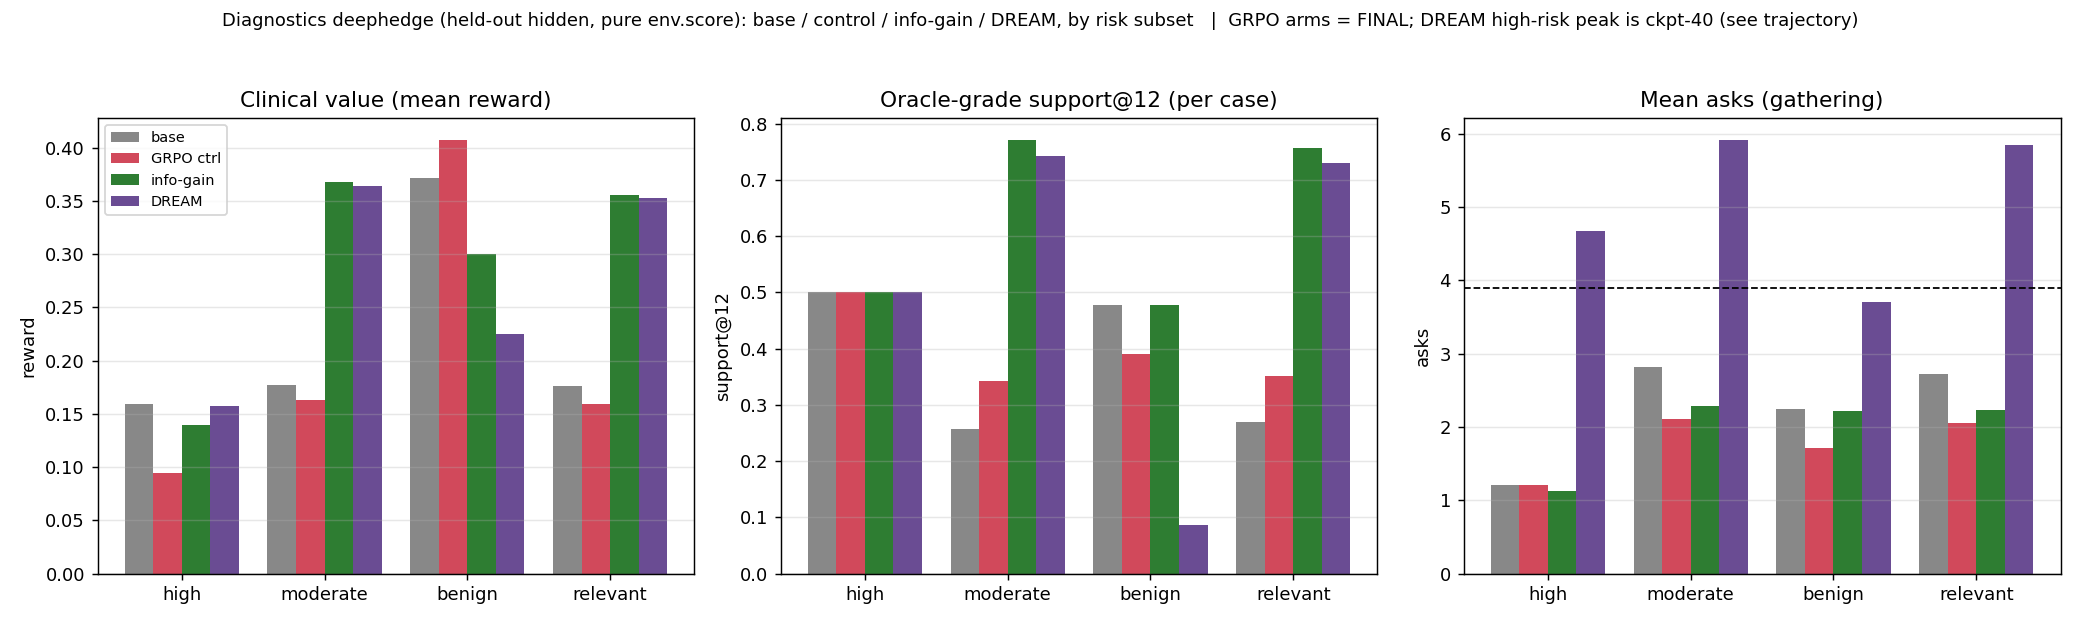
\includegraphics[width=\textwidth]{figs/dream_diagnostics_4arm.png}
\caption{Diagnostics by risk subset (held-out hidden, pure reward): base vs.\
plain-GRPO vs.\ info-gain vs.\ DREAM. Plain GRPO trims asks and regresses high-risk;
info-gain restores gathering and lifts the moderate subset; DREAM maximizes
high-risk oracle-grade support but over-gathers on low-acuity cases.}
\label{fig:dx4arm}
\end{figure}

\subsection{Decoupling further improves the safety-critical subset, at an
over-gathering cost}
Decoupling exploration from exploitation lets the explore policy gather without
commit-cost pressure and closes the VOI gap the single-policy reward left open:
mean asks rise from $2.2$ toward and past the oracle's $\approx 3.9$, and the
safety-critical high-risk subset improves markedly --- reward $+0.139 \to +0.248$
and oracle-grade support $0.50 \to 1.00$ at the best checkpoint
(Figure~\ref{fig:dreamtraj}) --- while still clearing all guards. The trade is that
the unconstrained explorer over-gathers on \emph{low-acuity} cases (benign support
$0.48 \to 0.04$) and overall value dips slightly below the info-gain policy. DREAM
thus delivers a favorable \emph{safety} trade rather than a strict domination: it
helps where gathering is decision-relevant and over-explores where it is not.

\begin{figure}[ht]
\centering
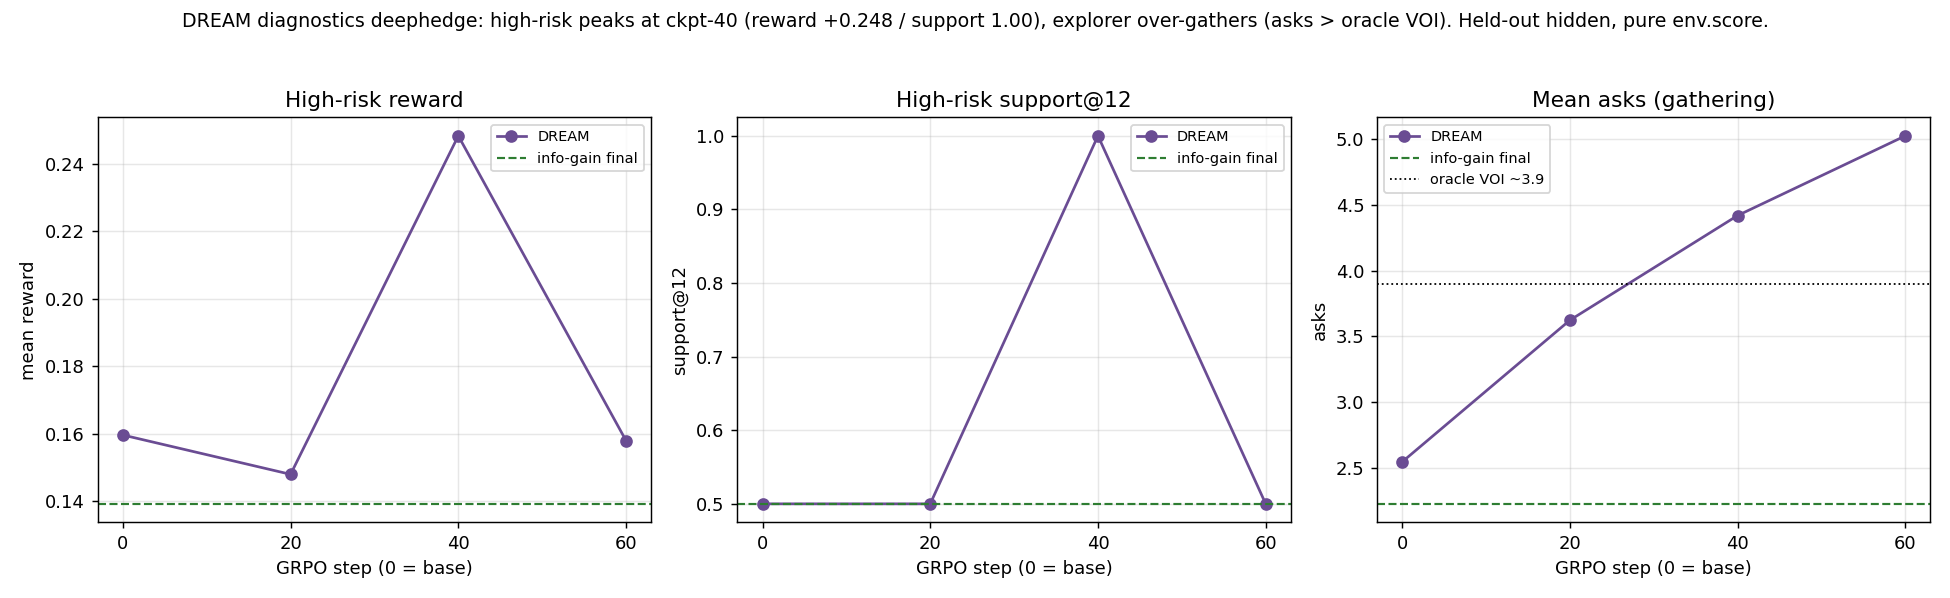
\includegraphics[width=0.92\textwidth]{figs/dream_diagnostics_trajectory.png}
\caption{DREAM checkpoint trajectory on diagnostics (held-out hidden, pure reward).
High-risk oracle-grade support and reward peak at checkpoint-40 (support $1.00$,
reward $+0.248$), above the information-gain reference, as mean asks rise toward
and past the oracle's $\approx 3.9$.}
\label{fig:dreamtraj}
\end{figure}

\subsection{The credit coefficient is a task-specific safety dial}
Titration --- a stylized ordered-intensity decision (no therapy / reduced / full)
under a clot-vs-bleed trade --- passes its gates (BC-gap $+0.075$; oracle uses all
three actions; gathering changes the committed action on $85\%$ of cases; optimal
intensity flips between clot-first and bleed-first priorities on $64\%$ of cases;
base latent support@12 $0.52$/$0.63$). The RL comparison (Table~\ref{tab:ti},
Figure~\ref{fig:tidial})
reveals a \emph{narrow} safe optimum for the credit coefficient, with failures on
both sides. Plain GRPO ($\lambda{=}0$) under-gathers (mean asks $2.8 \to 1.4$,
one-ask $0.91$, \textsc{exploit}). At the \emph{same} coefficient that was
thesis-positive on diagnostics ($\lambda{=}0.2$) the reward \emph{over-corrects}
into over-gathering (mean asks $4.1$, above the oracle's $\approx 2.8$), driving
overall value below base and control (\textsc{optimization-only}). At
$\lambda{=}0.03$ --- a first estimate matching the \emph{absolute} per-episode
shaping magnitude to diagnostics --- it \emph{under}-corrects, collapsing to one
ask like the control. The three points bracket the optimum. The correct scaling is
\emph{per ask}: a useful ask reduces posterior entropy by $\approx 0.33$ nats, and
the policy only gathers when the shaping offsets the per-ask cost ($0.03$), i.e.\
$\lambda\cdot\Delta H_{\text{ask}}\gtrsim c$, predicting $\lambda\approx0.1$. The
$\lambda{=}0.1$ run \emph{confirms the prediction on gathering}: it lands at mean
asks $2.67 \approx$ the oracle's $2.77$ with no one-ask collapse and no
over-gathering (consistently across checkpoints), and lifts high-clot oracle-grade
support to $1.00$ at sensible depth ($2.5$ asks, versus the control's hollow
$1.5$). Titration's larger information scale (nine joint states, prior entropy
$2.03$, per-episode information-gain $3\text{--}5\times$ diagnostics') is why a
single transferred $\lambda$ cannot serve both tasks: the credit-assignment
coefficient is itself a geometric quantity that must be calibrated to the per-ask
information-gain-to-cost ratio.

The calibrated coefficient, however, does \emph{not} convert into an overall
clinical-value win: $\lambda{=}0.1$ remains \textsc{inconclusive} (overall value
$-0.036$, support flat at base level). The reason ties reward geometry back to the
gates: titration barely clears Gate~1 (BC-gap only $+0.075$), so its value surface
is shallow and the ceiling on any value improvement is intrinsically low --- even
\emph{perfectly calibrated} gathering cannot manufacture headroom the task does not
have. This is a clean separation of the two factors: the credit coefficient
controls \emph{gathering behavior} exactly as the per-ask law predicts, but whether
better gathering yields a clinical-value win is governed by the task's
\emph{demonstrability headroom}. Diagnostics has a large BC-gap and converts;
titration has a marginal one and does not, despite identical machinery.

\begin{table}[ht]
\centering
\caption{Titration, held-out hidden condition, pure verifiable reward
(titration-aware subsets). The coefficient is a gathering dial: $\lambda{\le}0.03$
and plain GRPO \emph{under}-gather (one-ask collapse), $\lambda{=}0.2$
\emph{over}-gathers; the per-ask-predicted $\lambda{=}0.1$ lands at the oracle's
gathering level (asks $2.67$, no collapse) and lifts high-clot support to $1.00$.
But even calibrated gathering stays \textsc{inconclusive} on overall value, because
titration's BC-gap ($+0.075$) leaves little value headroom. High-clot value for the
collapsed policies ($\lambda{\le}0.03$, control) is a degenerate-policy artifact
(cheap one-ask aggressive commit), flagged \textsc{exploit} by the guard.}
\label{tab:ti}
\begin{tabular}{lccccc}
\toprule
Policy & overall value & overall asks & one-ask rate & high-clot value & high-clot supp \\
\midrule
base (untrained)                 & $-0.022$ & $2.76$ & $0.74$ & $+0.396$ & $0.67$ \\
plain GRPO (control)             & $-0.012$ & $1.40$ & $0.91$ & $+0.627$ & $1.00$ \\
\,+ info-gain ($\lambda{=}0.03$) & $-0.010$ & $1.24$ & $0.93$ & $+0.825$ & $1.00$ \\
\,+ info-gain ($\lambda{=}0.1$)  & $-0.036$ & $2.67$ & $0.62$ & $+0.556$ & $1.00$ \\
\,+ info-gain ($\lambda{=}0.2$)  & $-0.091$ & $4.10$ & $0.31$ & $+0.446$ & $0.67$ \\
\bottomrule
\end{tabular}
\end{table}

\begin{figure}[ht]
\centering
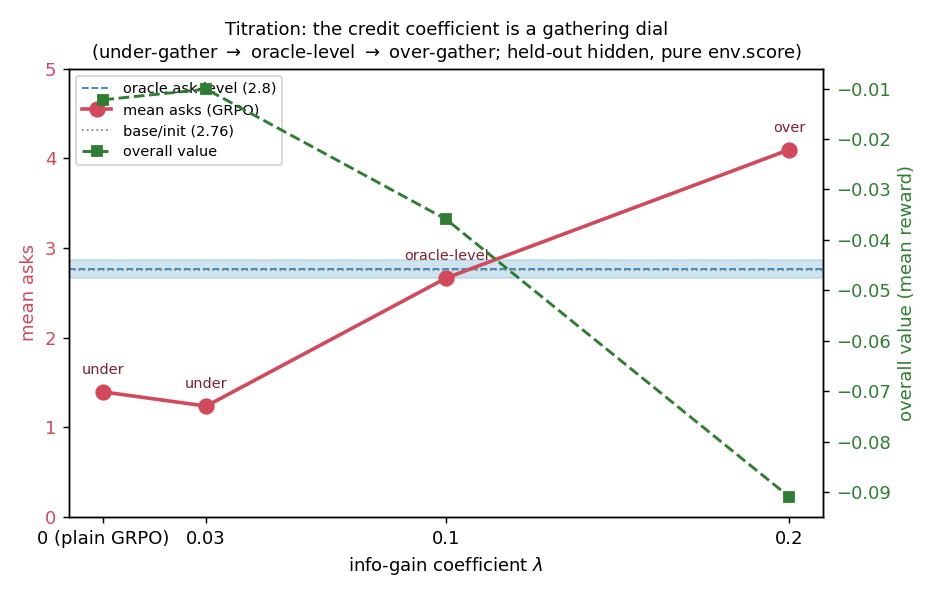
\includegraphics[width=0.7\textwidth]{figs/titration_lambda_dial.png}
\caption{Titration: the credit coefficient $\lambda$ is a gathering dial. Mean asks
(red) collapse below the oracle ask-level (blue band, $\approx2.8$) at
$\lambda{\le}0.03$, hit oracle-level at the per-ask-predicted $\lambda{=}0.1$, and
overshoot at $\lambda{=}0.2$; overall value (green) is best near the oracle-level
operating point. Held-out hidden, pure env.score.}
\label{fig:tidial}
\end{figure}

\subsection{Initialization matters: a saturated warmup leaves no headroom}
\label{subsec:bridge-result}
Refill triage is the one task whose RL starts not from base but from a \emph{light}
SFT warmup (the protocol-teaching gatherer of a prior multi-turn study, not a heavy
task-specific SFT). There, info-gain beats the plain-GRPO control at every
checkpoint (more asks, fewer one-ask shortcuts), and at the comparable early
checkpoint it \emph{preserves} high-risk reward at the warmup level ($+0.205$) where
the control has already crashed it ($-0.007$) --- but the benefit is transient and
no checkpoint reaches the strict thesis-positive bar
(Addendum Figures~\ref{fig:rx4arm}--\ref{fig:rxtraj}). The reason is that the
warmup --- though small --- already \emph{saturates} high-risk performance, leaving
no headroom for shaping to convert into a measured win; diagnostics and titration
instead train from base, where the headroom exists. This single SFT-initialized
case makes a concrete point that mirrors the titration BC-gap finding from the
other side: \emph{RL's payoff tracks the headroom left by the initialization}, just
as it tracks the headroom set by the task's demonstrability. We probe this
directly with a controlled coverage experiment next.

\subsection{SFT coverage: latent support is necessary but not sufficient for
repair}
\label{subsec:coverage}
To test the industrially common case of an SFT trained on incomplete data, we
build a deliberately \emph{coverage-biased} SFT on diagnostics --- oracle-adaptive
trajectories with the high-risk (emergent) cases under-sampled --- and ask whether
RL on the full environment repairs the resulting hole. The biased SFT illustrates
the central danger of aggregate metrics (Figure~\ref{fig:hole}): it looks excellent
overall (support $0.93$, value $+0.34$) while being \emph{unsafe} on the rare
high-risk cases (value $-0.29$; with all high-risk cases dropped, high-risk
support is $0.00$ and \texttt{emergent\_tx} is never emitted). A coverage gap is
thus hidden behind a strong headline score.

Crucially, the latent-support gate (Gate~2), \emph{re-measured on the biased SFT},
predicts whether RL can repair the hole. Severe bias (drop all high-risk) leaves
the high-risk action with $0\%$ sample rate --- Gate~2 fails, so RL has no signal
to reinforce. A milder bias (keep $30\%$) retains a $21\%$ \texttt{emergent\_tx}
sample rate --- Gate~2 passes --- so we run RL from it. Yet \emph{even with Gate~2
satisfied, RL does not repair the hole} (Table~\ref{tab:repair},
Figures~\ref{fig:reptraj}). The two variants fail in \emph{opposite} directions:
information-gain GRPO \textsc{exploits} --- it trims gathering ($3.0\to2.2$ asks)
and the high-risk oracle-grade support collapses ($1.00\to0.14$) into a defensive
hedge; DREAM \emph{over}-gathers ($3.0\to4.3$ asks, benign included), which damages
low-acuity cases (benign support $0.92\to0.16$) without restoring high-risk
support ($\to0.36$) and in fact lowers the \texttt{emergent\_tx} rate below the
SFT's. Both crash the SFT's strong overall support ($0.93\to0.41$). The pattern is
checkpoint-robust. This is the saturated-initialization regime of
Section~\ref{subsec:bridge-result} again: from a strong (if biased) SFT, RL erodes
the good behavior rather than targeting the hole. The conclusion is a sharp,
cautionary one: \emph{latent support is necessary but not sufficient for RL to
repair an SFT coverage gap} --- the initialization's strength and the reward
geometry determine whether RL repairs or merely re-shortcuts.

\begin{table}[ht]
\centering
\caption{SFT-coverage repair on diagnostics (held-out hidden, $n{=}200$, pure
verifiable reward). From a coverage-biased SFT that under-samples high-risk cases,
neither RL variant repairs the high-risk hole: info-gain collapses gathering (and
high-risk support) into a hedge; DREAM over-gathers and damages benign/moderate.
``supp'' is oracle-grade support@12.}
\label{tab:repair}
\begin{tabular}{lcccccc}
\toprule
Policy & overall val & overall supp & high val & high supp & benign supp & mean asks \\
\midrule
biased SFT (init)     & $+0.337$ & $\mathbf{0.93}$ & $-0.285$ & $\mathbf{1.00}$ & $\mathbf{0.92}$ & $3.0$ \\
\,+ info-gain GRPO    & $+0.236$ & $0.45$ & $+0.092$ & $0.14$ & $0.45$ & $2.2$ \\
\,+ DREAM             & $+0.292$ & $0.41$ & $+0.040$ & $0.36$ & $0.16$ & $4.3$ \\
\bottomrule
\end{tabular}
\end{table}

\begin{figure}[ht]
\centering
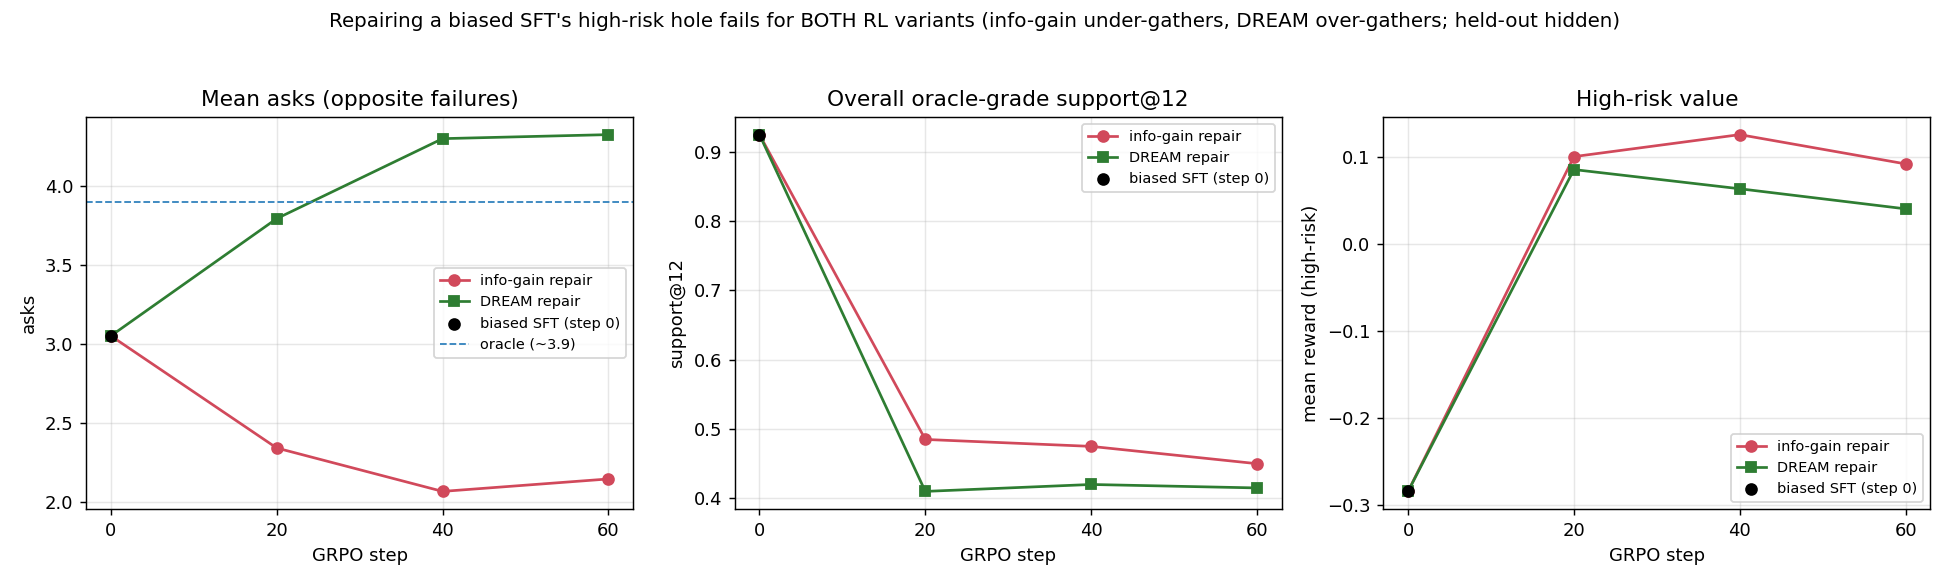
\includegraphics[width=\textwidth]{figs/repair_trajectory.png}
\caption{Repairing a biased SFT's high-risk hole fails for both RL variants. From
the biased SFT (step 0), info-gain trims asks down (under-gather) while DREAM
pushes them up past the oracle (over-gather) --- opposite failures --- and both
erode the SFT's overall support; high-risk value rises only marginally.}
\label{fig:reptraj}
\end{figure}

\begin{figure}[ht]
\centering
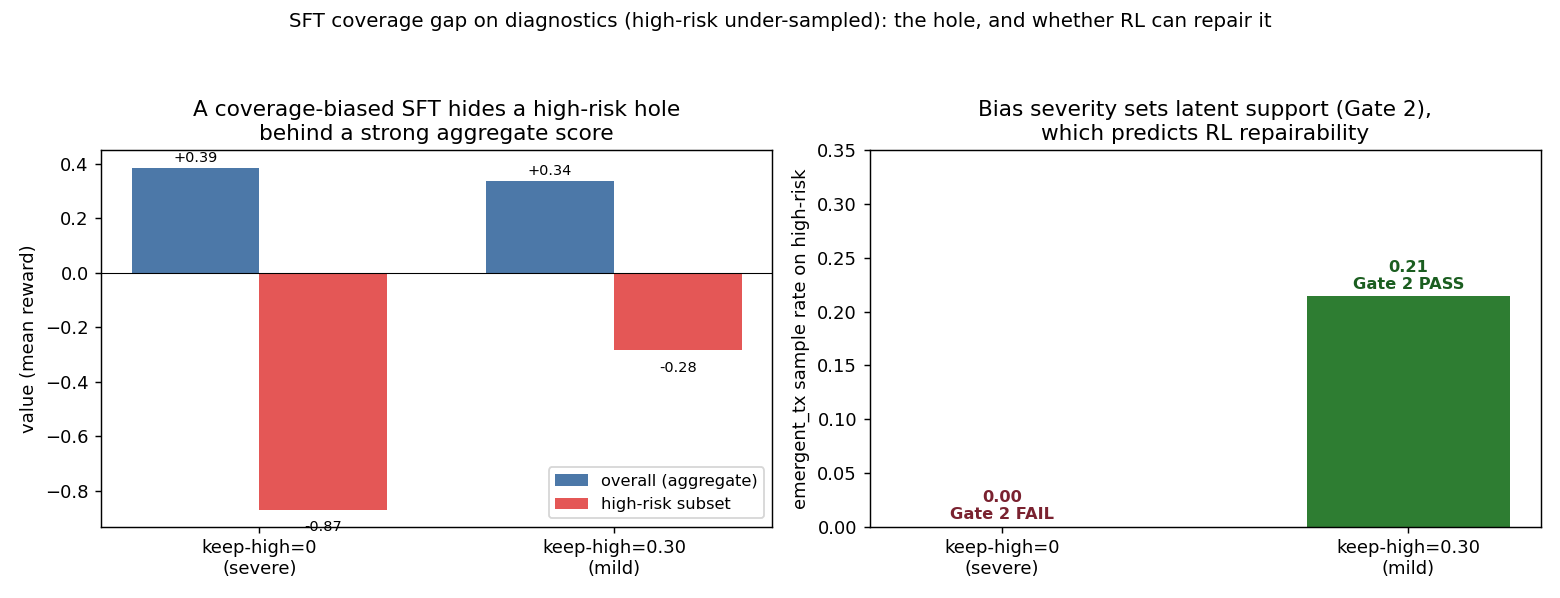
\includegraphics[width=0.92\textwidth]{figs/coverage_hole_gate2.png}
\caption{Left: a coverage-biased SFT looks strong on aggregate but is unsafe on
high-risk. Right: bias severity sets the high-risk action's latent support
(\texttt{emergent\_tx} sample rate), i.e.\ Gate~2 --- $0\%$ (fail) under severe
bias vs.\ $21\%$ (pass) under mild bias --- which predicts whether RL has any
signal to repair the hole.}
\label{fig:hole}
\end{figure}


\section{Discussion}
\label{sec:discussion}

\paragraph{A practical recipe.} The results compose into a decision rule for
post-training clinical gathering agents (Table~\ref{tab:guide}). The gates are
valuable as a \emph{negative} screen --- they predict where RL cannot help (no
BC-gap, or no latent support) so compute is not wasted --- but passing them does
not earn a win: with the plain outcome reward, GRPO learns unsafe shortcuts. The
controllable factor is \emph{reward geometry}. An information-gain
credit-assignment reward, applied purely in the RL rollout, restores safe adaptive
gathering where headroom exists; decoupling exploration from exploitation buys a
further high-risk-safety improvement at an over-gathering cost; and the credit
coefficient is a task-specific dial with a narrow safe optimum. The SFT-vs-RL
bridge adds the coverage axis: RL's payoff tracks the headroom the initialization
leaves.

\begin{table}[ht]
\centering
\caption{Practical guidance distilled from the experiments. ``Have'' = supported by
results in this paper; ``future'' = predicted by the framework and left to the
systematic SFT$\times$coverage study.}
\label{tab:guide}
\begin{tabular}{p{5.0cm}p{4.6cm}p{2.6cm}}
\toprule
Situation & Guidance & Evidence \\
\midrule
Demonstrability gate fails (a fixed action is near-optimal) & Do not run RL & analytic (have) \\
Latent-support gate fails (init cannot sample the optimum) & SFT/warm up first; RL has no signal & have (severe-biased SFT) \\
Gates pass, naive outcome reward & Expect unsafe shortcuts (1-ask, hedge, high-risk regression) & have (controls) \\
Gates pass, info-gain credit assignment, tuned coefficient & Safe adaptive gathering; calibrate $\lambda$ per task & have (diagnostics, titration) \\
High-risk safety is the priority & Decouple explore/exploit; accept some over-gathering & have (DREAM) \\
Task barely clears the demonstrability gate (small BC-gap) & Even calibrated RL yields little value gain & have (titration) \\
Strong/saturated SFT initialization & RL adds little --- no headroom to capture & have (refill triage) \\
Biased/incomplete SFT, Gate~2 passes & RL still may \emph{not} repair the hole --- it re-shortcuts from a strong init; do not assume repair & have (diagnostics coverage) \\
\bottomrule
\end{tabular}
\end{table}

\paragraph{Safety framing.} The headline is not ``RL improves medical reasoning''
but the sharper, safety-relevant claim that \emph{RL is not automatically safer}:
on the same gates-passing task, reward design determines whether the policy learns
adaptive gathering or exploits the verifier into an unsafe hedge or a one-question
guess. Because the damage concentrates in the rare high-risk subset and is masked
by mean reward, a pipeline that selects on aggregate reward can ship a less safe
policy --- which is exactly why the per-subset, guarded evaluation and the pre-RL
gates are the practical contributions.

\paragraph{Why clinical gathering is harder for RL than math or code.} The
reliable wins of RLVR have come from domains with a \emph{singular, unambiguous}
outcome --- a math problem is right or wrong, a program passes its tests or does
not \citep{shao2024deepseekmath} --- where the reward is simple, stable, and hard
to game. Multi-turn clinical decision-making has no such singular outcome: the
object of interest is a \emph{process} --- gather the decision-relevant facts,
weigh patient safety against burden, and commit only when enough is known --- so
the reward is subtler and shortcut policies (defensive hedging, under-gathering,
one-question collapse) are low-resistance attractors that score well on aggregate
while failing the cases that matter most. This reframes our cautionary results,
including the failed coverage-repair attempt, not as artifacts of a particular RL
implementation but as a property of the domain: in tasks where the reward is an
unambiguous endpoint, RL tends to help out of the box; in tasks where the reward
must encode a careful process, RL's value is contingent on reward design and on
actively screening for shortcut exploitation. The frontier for RL in nuanced
domains such as medicine is therefore reward and procedure design --- crediting
the gathering, not just the answer --- rather than raw RL capability, which is the
gap this paper's gates, credit assignment, and guarded evaluation are meant to
close.

\paragraph{RL shapes the inference procedure, not just the answer.} Our results fit
the same broader lesson as recent structured-inference work such as SPIRAL
\citep{hamid2026spiral}: RL does not merely change final-answer accuracy, it shapes
the inference procedure the model learns to execute. In our clinical setting the
failure mode is not redundant or poorly aggregated reasoning traces but unsafe
under-gathering, one-question collapse, and defensive hedging. Reward design
therefore has to target the clinical \emph{procedure} itself --- which facts are
gathered and when to commit --- not just the final answer. Together with OPSD-style
on-policy distillation \citep{zhao2026selfdistilledreasoner}, our results support a
broader view of post-training: the central problem is not simply SFT versus RL, but
how to convert verifiable or privileged information into dense credit assignment over
the inference procedure the model should learn. The success of applied systems such
as DoctorAgent-RL \citep{feng2026doctoragentrl} reinforces our central framing: in
clinical agents, the learned behavior of interest is not merely the final diagnosis
or action, but the information-gathering policy that produces it.

\paragraph{Limitations.} The environments are stylized, synthetic, and
rule-labeled with a deterministic simulator at a single 4B model scale, and the RL
runs are bounded; the contribution is a mechanism and a decision framework, not a
clinically validated policy. Headline results are single-seed; multi-seed
replication of the diagnostics thesis-positive result would further harden them. For
diagnostics and titration we characterize RL \emph{from base}; the SFT-initialized
evidence is two cells (a light warmup on refill triage and a coverage-biased SFT on
diagnostics), without an SFT-dose/saturation sweep, so our SFT-coverage claim is a
demonstrated failure-to-repair under a strong biased init, not a full
characterization across SFT strengths.

\paragraph{Future work.} The natural next study is the full
\emph{coverage}$\,\times\,$\emph{demonstrability} matrix. The complement to our
biased-SFT cell is a \emph{strong}-SFT$\to$RL cell (full SFT on oracle trajectories
on a demonstrable task --- does RL still add once SFT has plateaued?) with an
SFT-dose curve to establish saturation, and a weaker-init biased cell to test
whether repair is possible when the initialization is \emph{not} already saturated.
The larger version adds \emph{non-demonstrable} task
variants (stochastic patient responses, hidden confounders, ambiguous stopping)
where no static demonstration captures the optimal policy and RL should retain value
even after strong SFT. Two further extensions of the present machinery are gated and
designed:
\emph{goal-conditioned} adaptive gathering (conditioning the policy on a stated
safety/burden/control priority, with the optimal action and the amount of gathering
shifting with the goal) and analytic \emph{hindsight relabeling}
\citep{andrychowicz2017her} for sample efficiency, exploiting the analytic verifier
to rescore a trajectory under alternate goals. These build directly on the gated,
reward-geometry-aware foundation established here.

\section*{Addendum: refill-triage figures}

\begin{figure}[ht]
\centering
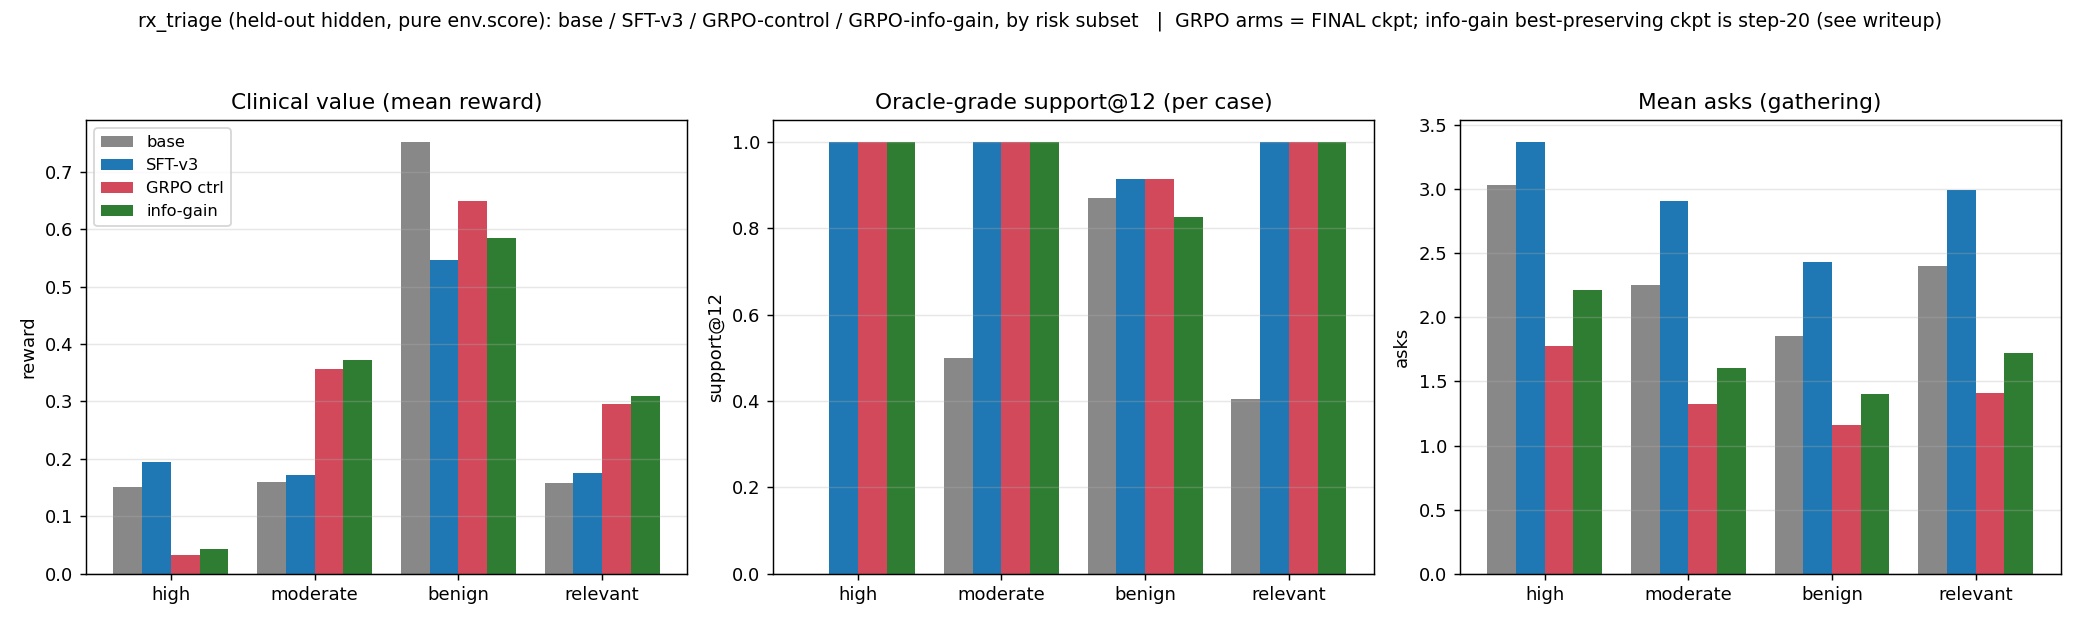
\includegraphics[width=\textwidth]{figs/infogain_rx_base_sft_ctrl_ig.png}
\caption{Refill triage by risk subset (held-out hidden, pure reward): base /
SFT-v3 warmup / GRPO-control / GRPO-info-gain (final checkpoints). At the endpoint
both GRPO arms erode high-risk relative to the SFT warmup, which already saturates
it.}
\label{fig:rx4arm}
\end{figure}

\begin{figure}[ht]
\centering
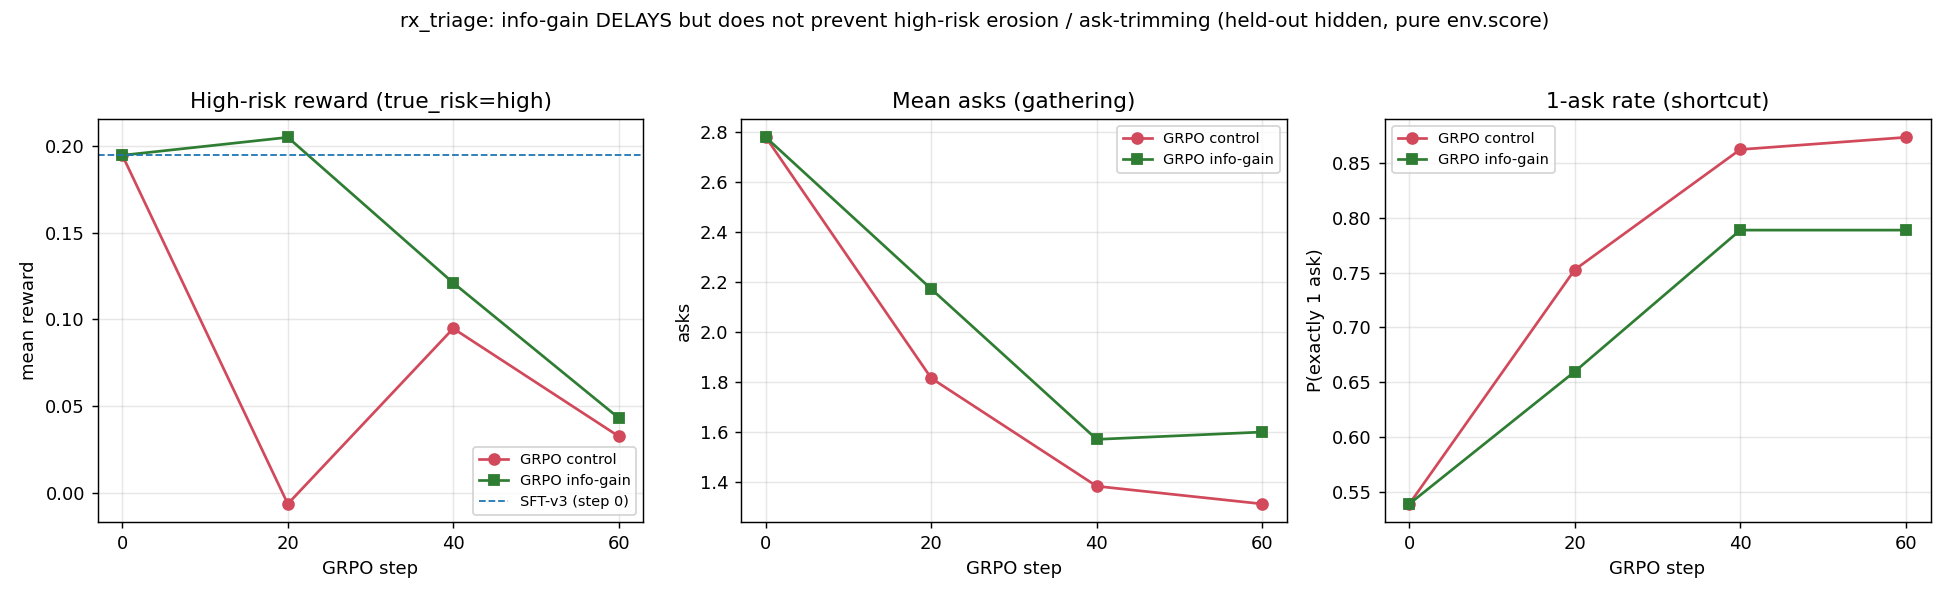
\includegraphics[width=0.92\textwidth]{figs/infogain_rx_checkpoint_trajectory.png}
\caption{Refill-triage checkpoint trajectory, GRPO-control vs.\ GRPO-info-gain.
Info-gain preserves high-risk reward at the warmup level at step-20 ($+0.205$)
while the control has already crashed it ($-0.007$); the benefit is transient as
both trim gathering with continued training.}
\label{fig:rxtraj}
\end{figure}

\begin{figure}[ht]
\centering
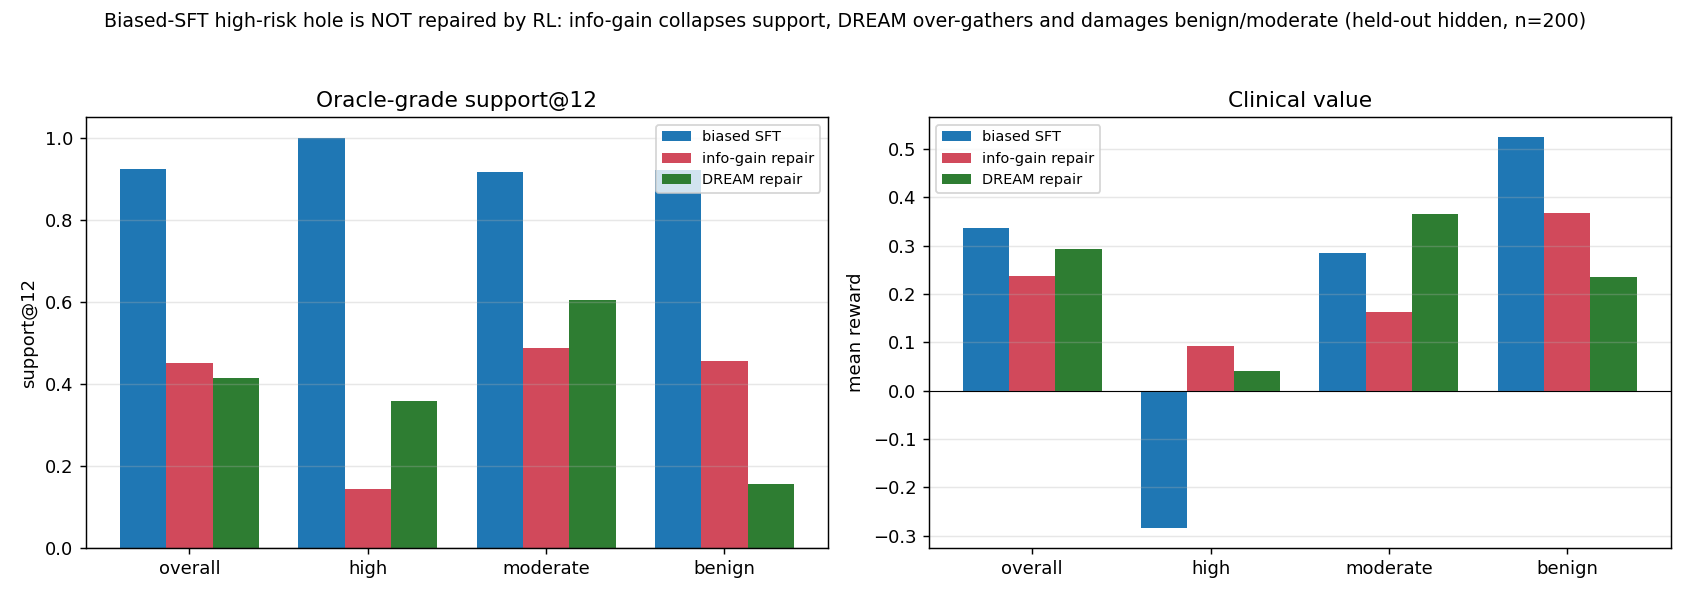
\includegraphics[width=\textwidth]{figs/repair_4arm.png}
\caption{SFT-coverage repair by risk subset (held-out hidden, $n{=}200$): biased
SFT vs.\ info-gain-repair vs.\ DREAM-repair. Neither RL variant restores high-risk
oracle-grade support ($1.00\to0.14$ info-gain / $0.36$ DREAM); DREAM additionally
collapses benign support ($0.92\to0.16$) by over-gathering. Companion to
Table~\ref{tab:repair} and Figure~\ref{fig:reptraj}.}
\label{fig:rep4arm}
\end{figure}

\section*{Code}
\url{https://github.com/csbrendan/rl-gains-in-clinical-tasks}

\label{sec:cite}
\bibliography{sample.bib}
\bibliographystyle{plainnat}

\clearpage
\end{document}
